\chapter{Edges}
\label{sec:edges_background}
\begin{figure}
    \centering
    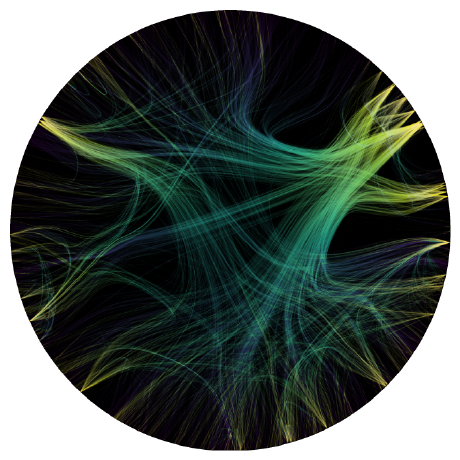
\includegraphics[width=\textwidth]{power/figures/metaunityplaceholder.png}
    \caption{A visualisation of the Unity game engine, produced using the Unity game engine. TODO: explanation of hierarchy and labels around perimeter. Also move this to the start of the chapter}
    \label{fig:metaunity}
\end{figure}
The previous chapter of was an exploration of how to position the vertices of a graph, and the natural question to then ask is how to deal with the only remaining component: the edges. However this question is seemingly redundant at first, as the obvious answer is to simply draw straight lines between adjacent nodes. While this by no means a poor choice, and is exactly how all node-link diagrams have been drawn thus far, this chapter will explore the possibility of drawing links using curves instead.

\section{Background}
The curving of links in the context of a node-link diagram is known as \textit{edge bundling}. It is a technique that has been developed because many networks, when processed through a standard force-directed layout, result in a seemingly random layout with no discernable structure. See Figure~\ref{fig:untangled_hairballs} for an example. The similarity of such layouts to tangled piles of hair has led to them being colloquially termed \textit{hairballs}.

Unfortunately this is not an easily solved problem, because the \textit{curse of dimensionality} \cite{Friedman2001} means that most of these networks simply cannot be accurately represented in two dimensions, and the likelihood of this problem only rises as the size of any network increases. This is all even if there is a clear underlying structure to these networks, lying beyond the reach of the standard layout algorithm.
Edge bundling attempts to alleviate this issue by introducing a trade-off---the ability to follow individual links is sacrificed for better representation of global structure, by allowing links to overlap.
This is analogous to organising the wires in a computer system by tying groups of wires together that share similar endpoints.

The literature is rich with various different methods for performing this bundling, dating all the way back to the 1800s with the flow maps of Minard \cite{Minard1862} or Sankey diagrams \cite{Sankey1896}.
More modern algorithms for performing bundling automatically include multilevel agglomerative edge bundling (MINGLE) by Gansner et al.\ \cite{Gansner2011} which greedily merges pairs of links at a time by selecting the pairs that minimise a cost function based on the amount of `ink' used to draw links. A more complex cost function is used in metro-style bundling by Pupyrev et al.\ \cite{Pupyrev2016}, which is based on multiple criteria including ink, individual edge lengths and node separations. 
The same premise behind force-directed node layout is also used in force-directed edge bundling by Holten and van Wijk \cite{Holten2009}, which bundles links by defining forces between adjacent links instead of nodes. As shown previously in Section~\ref{sec:force_background}, force-based methods are in fact gradient descent optimisation methods where the gradient is defined before the cost function itself, and this edge bundling technique is no different.

Another effective approach is \emph{kernel density estimation} by Hurter et al.\ \cite{Hurter2012}, who iteratively apply a convolutional filter over a density map of links in an already rendered diagram. This method belongs to the subfield of image-based bundling methods \cite{Lhuillier2017,Telea2018}. A diverse gallery of edge bundling algorithms applied to the same dataset can be see in the review of Lhuilier et al.\ \cite[Fig.~4]{Lhuillier2017}.
However all of the aforementioned methods share a key similarity: they apply bundling upon the assumption that node positions are predetermined and will not be moved. This is perfectly fine and even desirable in many common use cases where nodes have a predefined location, such as geographical maps, but methods such as force-directed layouts were never designed to place similar edges in parallel. In fact, the angular resolution of edges sharing nodes is sometimes used as part of the optimised cost function \cite{Argyriou2010}) and so common layout methods usually do not help, if not worsen, the bundling quality of their visualisations.

This is why one of the most powerful network visualisation techniques is method known as \emph{hierarchical edge bundling}, published by Holten in 2006 \cite{Holten2006}\footnote{Its effectiveness was recognised by a `Test of Time' award at the IEEE VIS conference in 2016.}
An example of this in action can be seen in Figure \ref{fig:metaunity}, which contains the method applied to the source code of the Unity game engine. The graph being visualised is a call graph, where each class is a vertex, and is connected by an edge to any other class it depends on. 

The trick to the bundling comes from the fact that we have extra metadata available: the hierarchy of folders and source files that holds the code.
This hierarchy, not the call graph itself, is first layed out as a tree. Then, since this tree includes extra nodes to represent the folders and source files, these extra nodes are erased from the final visualisation. However their coordinates are instead used as an auxiliary routing graph (ARG) through which the call graph edges are routed through.
More precisely, this process of routing involves taking every edge in the call graph, and rendering each one using a spline curve whose control points consist of a path through the ARG. The precise definition of this spline is important, and will be further elaborated upon in Section~\ref{TODO}, but for now the important thing to note is that this produces bundling behaviour because vertices close to each other in the hierarchy will share control points for their splines, thus curving their rendered links towards each other.
The hierarchical tree extracted from the Unity game engine can be seen on the TODO hand side, to illustrate its influence on the final visualisation. 

This technique is so effective because the structure of the bundles is informed by human judgement. To continue within the call graph example, the hierarchy of folders and source files is literally designed by the programmers for organisational purposes, and so it is very likely to admit some utility for also organising, say, a visualisation.
Additionally, not only is the curvature links influenced by the ARG, but so is the position of the nodes. Since each node is a leaf in the tree-shaped ARG, their positions around the circle are also influenced by the topology of the tree, which on its own already vastly improves the quality of the layout.
This idea of using an auxiliary hierarchy to inform bundling is the basis of the work in this chapter, except that I will instead investigate the more common situation of when this metadata is not included with the original data. It must therefore must be generated by the algorithm itself as a preprocessing step.

\subsection{Clustering}
What is needed is a way of grouping similar datapoints together. This is known as \textit{clustering}, and is a vast field of study, not least as one of the primary objectives of the fast-growing discipline of machine learning. The subfield of clustering just within the context of networks is large in its own right, due to its utility in common datasets such as protein--protein interaction or social networks.

There exist a wide variety of powerful and creative methods that have been developed to perform clustering on networks. A widely used method is to define an equation that can be used to numerically measure the quality of a given clustering, and to attempt to maximise this quality. This is reminiscent of the optimisation-based methods described in Section~\ref{sec:force_background}.
A popular version of this is known as \emph{modularity}, defined as
\begin{equation}
    Q = \frac{1}{|E|}\sum_{i,j}\left(\mathbf{A}_{ij} - \frac{|N(i)||N(j)|}{|E|}\right)\mathbf{C}_{ij}
\label{eq:modularity}
\end{equation}
where $\mathbf{A}$ is the adjacency matrix where $\mathbf{A}_{ij}$ equals 1 if vertices $i$ and $j$ are connected by an edge, and $\mathbf{C}_{ij}$ equals 1 if vertices $i$ and $j$ are in the same cluster and 0 otherwise.
The value of $Q$ lies between $\text{--}\sfrac{1}{2}$ and 1 \cite{Brandes2007a}, and it can be intuitively understood as the fraction of the edges that fall within the given clusters minus the expected fraction if edges were distributed at random.

This was introduced by Newman and Girvan \cite{Newman2004} to evaluate a separate clustering algorithm, and later directly optimised by Newman \cite{Newman2006} with two methods that both initialise the network as one big cluster that is recursively split into half until no further gain in modularity is possible. The first finds the split by calculating eigenvectors of the \emph{modularity matrix}, and another that finds the split by repeatedly moving vertices between the two sides of the split until modularity is maximised, akin to a hill-climbing method.
Optimising modularity in general is $\mathcal{NP}$-complete \cite{Brandes2007a}, but its intuitive interpretation has led to various other authors to develop methods to optimise it. The Louvain algorithm (given its name from the authors coming from the University of Louvain, Belgium) \cite{Blondel2008} and its recent improvement to the Leiden algorithm (from Leiden University, Netherlands) \cite{Traag2019} both start by placing every vertex in a singleton cluster and successively merging clusters whilst also moving vertices between clusters, also until modularity cannot be improved further.

The behaviour of random walks along the graph has also been used to great effect for clustering. For example, the \emph{markov cluster} algorithm of Enright et al.\ \cite{Enright2002} simulates a random walk process through a series of matrix multiplications on the markov chain of the graph.
The \emph{infomap} algorithm of Rosvall and Bergstrom \cite{Rosvall2008} optimises a cost function known as the map equation, which applies information-theoretic concepts such as entropy to the behaviour of random walkers. It is optimised through a combination of greedy search and simulated annealing.
Other types of algorithms include statistical inference methods such as Bayesian inference \cite{Hastings2006} and block-modelling \cite{Reichardt2007}.
Another perspective on clustering includes grouping together edges instead of vertices, which means that a single vertex may belong to many overlapping clusters, an idea explored by Evans and Lambiotte \cite{Evans2009}.
The growing number of graph-shaped datasets being used in machine learning has also led to a number of supervised and semi-supervised methods for clustering and general dimensionality reduction, such as \emph{DeepWalk} \cite{Perozzi2014} which treats each vertex as a `word' to generate `sentences' using random walks across vertices. These sentences are then taken and applied to techniques originally designed for language processing. Attempts to transfer the success of convolutional neural networks have also been generalised to apply to graphs of any topology \cite{Kipf2016, LeCun2017}, as well as many other architectures depending on the task at hand \cite{Battaglia2018, Wu2020}.

% The variety of different methods available is in part due to one key characteristic of network clustering: it is an undefined problem.
One reason why there is such a variety of clustering algorithms is due in part to it being an undefined problem.
Clustering can be likened to data compression, as the goal is to describe a given network with less information than, say, viewing the source and target of every individual edge. Such compression would be impossible in a random network, but because real-world data does have structure, underlying patterns can be leveraged to group together similar components within the data.
However, even knowing that this is the goal does not make the problem easier, because these underlying patterns are not known to us. The real world is complex, and so any data collected from it is not likely to be straightforward to understand. Much of the data collected may not even contain any order in the first place.
% In fact, if you will allow me to go meta for a moment, the very act of collecting data itself into the form of a network is already technically a form of compression, as 
It is therefore important to keep in mind that clustering algorithms are attempts to quantify common characteristics of real-world data, and there is generally no `right answer' to the question of which one should be chosen.
It depends on both the specific objective and dataset being examined. Nevertheless, they have been used to great effect in many applications \cite{Fortunato2016}, and so confidence can be placed in their utility as a tool to help understand patterns in data.

The work in this chapter will focus on \emph{hierarchical clustering}, the family of clustering algorithms where the output is a \textit{dendrogram}: a binary tree used to describe a hierarchical structure.
This can either be done from the bottom up, i.e.\ each node starts in its own cluster and pairs of clusters are progressively merged until only one remains, or top down, i.e\ every node starts in the same cluster that is recursively split into two halves. The former is known as \emph{agglomerative} clustering, and the latter as \emph{divisive} clustering.
The output fits well with our purposes, since our goal is to construct a hierarchical edge bundling visualisation like the one in Figure~\ref{fig:metaunity}, but without a prior hierarchy included with the data; the dendrogram produced from such a clustering algorithm can be used as this missing hierarchy.

This idea of using the output dendrogram of a clustering algorithm to produce hierarchical edge bundling has been previously explored by Jia et al.\ \cite{Jia2011}\footnote{TODO: bad splines} who produce a hierarchy using the algorithm of Girvan and Newman \cite{Girvan2002}. This method removes one edge from the network at a time, specifically the one with the most \emph{betweenness centrality} i.e.\ the edge traversed the most often when mapping the shortest paths between all pairs of vertices. This naturally splits clusters when an edge is removed that is the final bridge between two clusters.
Unfortunately Jia et al.\ did not perform any quantitative analysis to evaluate the performance of their clustering algorithm, and only present results when using one clustering method. The work in the following section will aim to extend their work by evaluating the performance of a number of hierarchical clustering methods, against a benchmark of graphs where the ground truth cluster configuration is known.

\section{Hierarchical Clustering}
\begin{figure}
    \centering
    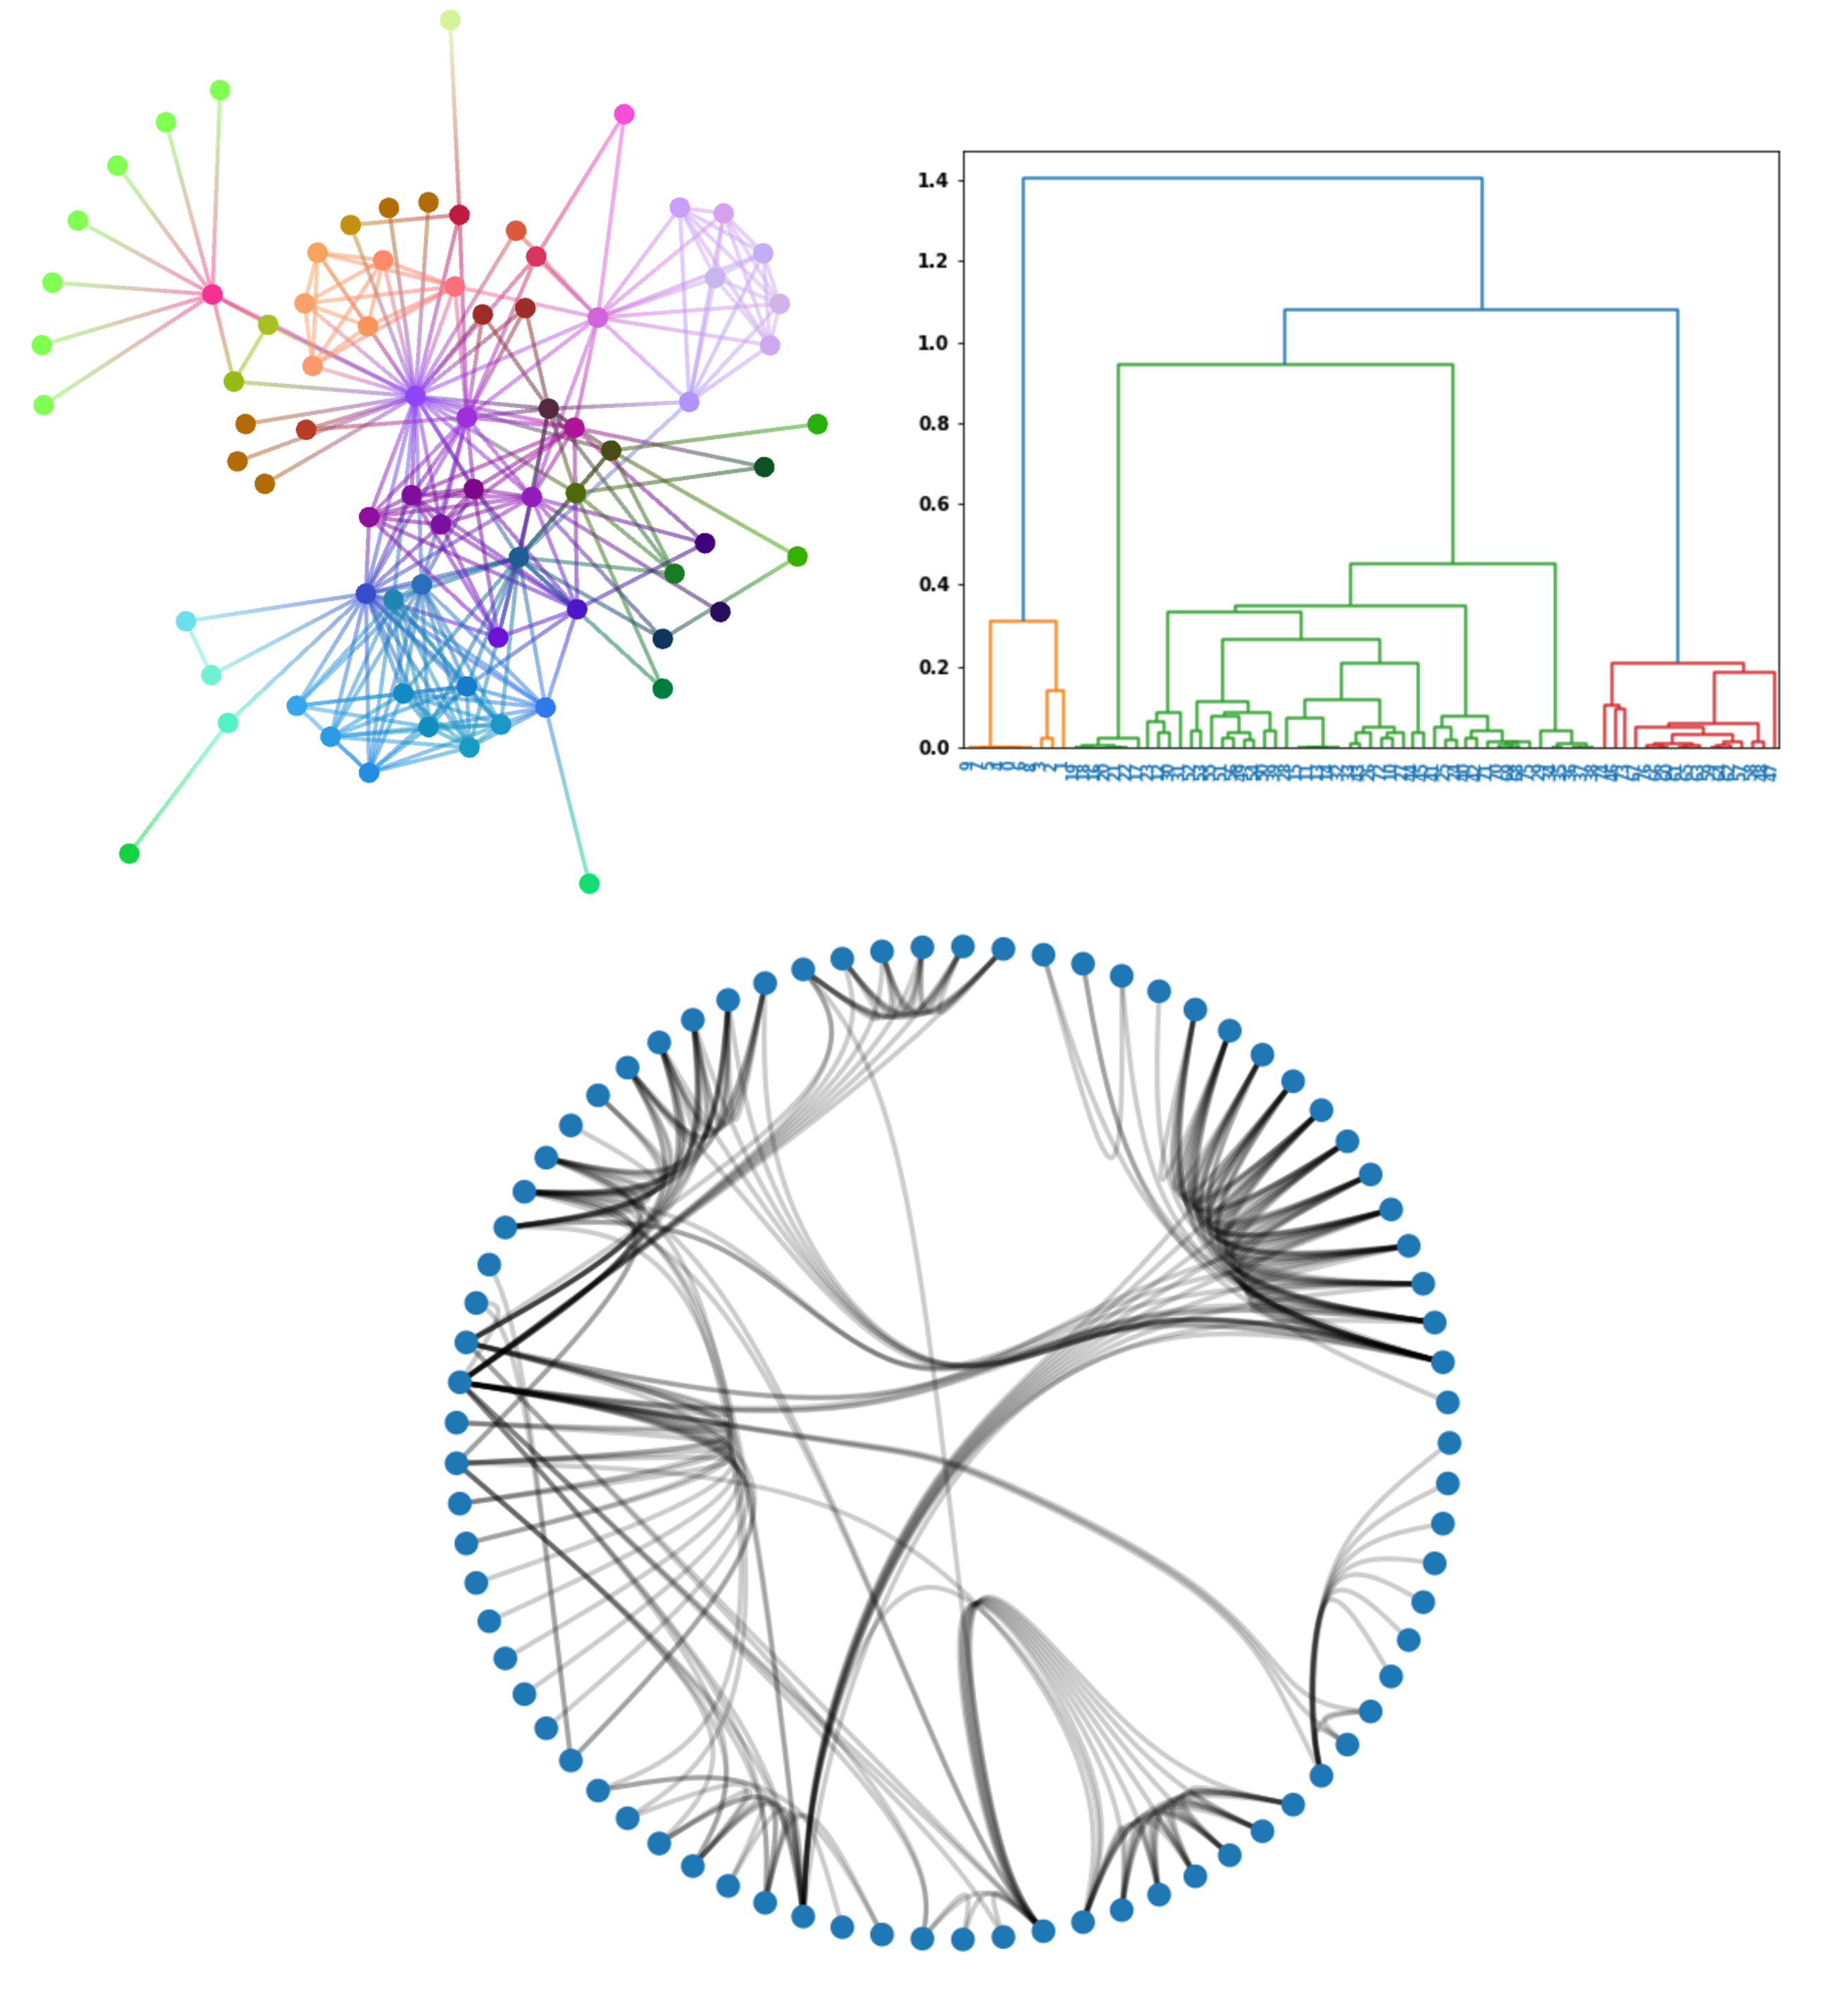
\includegraphics[width=\linewidth]{power/figures/lesmis.pdf}
    \caption{An example of the target: edges have weights, todo: move circle to bottom with plus sign}
    \label{fig:lesmis}
\end{figure}
To assess the quality of the divisive Girvan-Newman algorithm used by Jia et al.\ \cite{Jia2011}, it will be compared with \emph{agglomerative dissimilarity clustering}.
This is a family of algorithms where the input is a matrix of \emph{dissimilarities} between individual datapoints, in this case the vertices of a graph, and the output is a dendrogram as required. Similarly to the stress-based layout explored in the previous chapter, it is a more general algorithm that can be applied to any numerical datasets and not just graphs, unlike the methods previously outlined in Section~\ref{sec:edges_background}. It is also closely related to the class of multidimensional scaling methods that stress minimisation belongs to, as both procedures take a matrix of dissimilarities as input.

Not only does this fit thematically with the topics explored in previous chapters, but a key benefit to using dissimilarity clustering is that the output dendrogram contains extra information to describe the `quality' of the merge at that point. This information is vital as it can be used to `prune' the hierarchical tree in order to make the resulting edge bundles more salient. This will be elaborated upon in Section~\ref{sec:pruning}.
Two other questions must first be answered before we can proceed with performing this clustering: what exactly are the dissimilarities to be used as our input, and how will the algorithm proceed to process these dissimilarities to merge clusters? These will both be answered in the following section.

\subsection{Dissimiliarity Clustering}
\label{sec:dissimilarities}
General hierarchical clustering based on dissimilarities can be done in both an agglomerative and divisive way, but the work here will focus on agglomerative methods. Agglomerative methods are more popular among practitioners \cite{Roux2018} due largely to the divisive version having $\mathcal{O}(2^n)$ possible splits for a cluster of size $n$, as each datapoint can be placed in either one half or the other. This results in an exponential runtime complexity per split, whereas the agglomerative method has only to chose from pairs of datapoints, giving an $\mathcal{O}(n^2)$ complexity per merge.

There do exist heuristics to speed up the divisive method to bring the complexity down to polynomial, such as using algorithms like k-means to decide the split instead \cite{Lamrous2006}.
% It can also be argued that a divisive method can take a more global approach.
However, since we already have a graph-specific divisive method in the Girvan-Newman algorithm to compare to, the work on this chapter will focus on comparing it to its agglomerative counterparts.

\subsubsection{Greedy Agglomeration}
The agglomerative process is as follows:
\begin{mdframed}[backgroundcolor=WhiteSmoke]
\begin{enumerate}[leftmargin=*]
    \item Calculate the dissimilarities between all pairs of datapoints. \label{item:agglomerate_calculate}
    \item Place each datapoint into its own singleton cluster.
    \item Iterate over each pair of clusters, and merge the closest pair into a single cluster. \label{item:agglomerate_pairs}
    \item Recalculate the dissimilarities between the newly merged cluster and the remaining unmerged clusters. \label{item:agglomerate_recalculate}
    \item Repeat steps \ref{item:agglomerate_pairs} and \ref{item:agglomerate_recalculate} until only one supercluster remains.
\end{enumerate}
\end{mdframed}
On the surface this is a simple procedure, but it is not immediately clear how to calculate dissimilarities between datapoints or between clusters in steps \ref{item:agglomerate_calculate} or \ref{item:agglomerate_recalculate}.
There are an abundance of choices for what to use for step \ref{item:agglomerate_calculate}, which is the same first step as used in stress-minimisation from Section~\ref{sec:stress_background}. There, the graph-theoretic shortest-path was used as the dissimilarity, but there exist a wide variety of other measures that can be used that result in higher quality results. This will be shown in the experimental comparison in Section~\ref{sec:clustering_experiment} and discussed later in this section. Here I will start by assuming that we have a dissimilarity already defined between datapoints, and discuss how they are recalculated when clusters are merged.

There are also many choices for recalculating dissimilarities between clusters, and each choice can be thought of as a different heuristic for the greedy choice of which pair of clusters to merge together.
The most commonly used methods fall into three categories: using one member of a cluster as a representative, averaging over all cluster members, and measuring the variance of members within a cluster \cite{Roux2018}.
Choosing a single representative member is the most straightforward; when calculating the dissimilarity between two clusters, one can take the best-case scenario by choosing the closest pair of inter-cluster points, or the worst-case by choosing the farthest pair. These are known as single- and complete-linkage algorithms, respectively \cite{Sibson1973, Defays1977}.
One can also choose to take an average over the members of both clusters. This can be done by taking the mean dissimilarity between all inter-cluster pairs, and and is known as UPGMA (Unweighted Pair Group Method with Arithmetic mean). Its `weighted' counterpart, known as WPGMA, is more efficient, as when a cluster is merged it `forgets' that it was made up of other elements and becomes treated as a single datapoint itself \cite{Sneath1973}. The reason it is called weighted is, perhaps confusingly, because the original datapoints `lose weight' by being merged into a cluster, whereas in the unweighted version each original datapoint still contributes the same amount to each merging decision.

The third category is known as the Ward method, and is based on minimising variance within clusters. The dissimilarity between clusters in this case is the increase in total within-cluster variance if they were to be merged. This is the same objective function that k-means clustering attempts to minimise \cite{Friedman2001a}.
\footnote{The best description of these types is the shape of clusters. single linkage is an amoeba, complete is a hypersphere, upgma is, wpgma, ward is a 'type' see \url{https://stats.stackexchange.com/questions/195456/how-to-select-a-clustering-method-how-to-validate-a-cluster-solution-to-warran/195481\#195481}}

Note that since each merge is based on the dissimilarity between clusters, this extra information that can be stored in the resulting dendrogram as the height of the branch. This is a direct benefit of using dissimilarity clustering, and is usually used to decide where to cut the dendrogram if flat clusters are needed. It will be leveraged to simplify the resulting dendrogram in Section~\ref{sec:pruning}.
However this is also a source of trouble for Ward's method specifically, because a monotonically increasing branch height is only guaranteed if the input is a \emph{distance}, and not just a \emph{dissimilarity}.
A distance must strictly satisfy the conditions
\begin{equation}
\begin{aligned}
    d_{ij} & \geq 0 \quad\mathrm{and}\quad d_{ij}=0 \Leftrightarrow i=j \\
    d_{ij} & = d_{ji} \\
    d_{ij} & \leq d_{ik} + d_{ky}
\end{aligned}
\end{equation}
where the third condition is known as the triangle inequality, and is a requirement for the points to have a corresponding embedding in a metric space, such as Euclidean.
A dissimilarity is only required to satisfy the first two conditions.
Since Ward's method is based on variance, a concept that only makes geometric sense in a metric space, using a dissimilarity may result in dendrograms with negative branch lengths, making it impossible to cut the tree and form flat clusters.

The results in Section~\ref{sec:clustering_experiment} will include both distances and dissimilarities, both applied to Ward's method and the others reviewed in this section.
In practice, any reasonable dissimilarity does not often result in negative branch lengths with Ward's method, even if it does not satisfy the criteria of a distance. None of the results presented on the benchmark used here have this problem, but it is important to note the possibility of it happening in practice.

The final thing to discuss before moving onto how to choose a dissimilarity is the computational complexity on recalculating dissimilarities between clusters when they are merged. Remarkably, all of the above methods can be recalculated based on the equation
\begin{equation}
    \;d_{\{i\cup j\}k} = \alpha_i d_{ik} + \alpha_j d_{jk} + \beta d_{ij} + \gamma|d_{ik}-d_{jk}|
\end{equation}
where $d_{\{i\cup j\}k}$ is the new distance between $k$ and a newly merged cluster containing $i$ and $j$. The values of $\alpha$, $\beta$, and $\gamma$ can all be calculated in constant time.
Recalculating the dissimilarity matrix after a merge therefore takes $\mathcal{O}(|V|)$ time. Searching through this matrix to find the best merge takes $\mathcal{O}(|V|^2)$ time, but this can be reduced to $\mathcal{O}(|V|\log(|V|)$ with a priority queue. Since forming a complete dendrogram requires $\mathcal{O}(|V|)$ merges, the overall complexity of greedy agglomerative clustering is $\mathcal{O}(|V|^2\log(|V|)$ .


\subsubsection{Random Walks as Dissimilarities}
The first step before performing the agglomeration is to calculate the pairwise dissimilarities between individual datapoints. As previously noted, the shortest path distance was used in the context of optimising stress, but it be shown here that this is far from optimal in a clustering context.
The reason for this that there is not enough \emph{local} information to differentiate vertices successfully.    
For example, imagine a graph with two fully connected cliques, but with one edge connecting a single inter-cluster pair. Since the shortest path between the pair is one hop, it means that the pair is considered just as similar to each other as to the other vertices in their respective cliques.
Similarly, in a biclique vertices in the same group are not connected at all, and so within-cluster pairs would be considered even less similar than inter-cluster pairs.
% These examples are illustrated in Figure~\ref{fig:bacon_bad}.
% \begin{figure}
%     \caption{TODO: show why bacon is bad with 2 cliques and a biclique}
%     \label{fig:bacon_bad}
% \end{figure}

A commonly used distance to capture local detail is the Jaccard index
\begin{equation}
    d_{ij} = 1 - \frac{|N(i) \cap N(j)|}{|N(i) \cup N(j)|}
\label{eq:jaccard}
\end{equation}
which can be interpreted as the proportion of neighbours shared between vertices $i$ and $j$. However, this has the exact opposite problem to using shortest paths, as it fails to capture any \emph{global} detail, because any pair of vertices more than two hops away can never share any neighbours, and so will always have a maximum dissimilarity of one.
An ad hoc solution to this problem is to combine the two measures by simply multiplying them together, following Zheng et al.\ \cite{Zheng2018}. Note that despite shortest paths and Jaccard index both being distance metrics \cite{Clarkson2006}, it is not guaranteed the resulting dissimilarities will also be.

A popular method of graph clustering that uses dissimilarities as input is the \emph{cluster walktrap} method of Pons and Latapy \cite{Pons2006}. They use \emph{random walks} to first construct a high-dimensional embedding of each vertex.
To construct the high-dimensional embedding, the \emph{Markov chain} transition matrix of the graph is calculated, defined as
\begin{equation}
    \mathbf{P} = \mathbf{D}^{-1} \mathbf{A}
\end{equation}
where $\mathbf{D}$ is a diagonal matrix of degrees, where the entries are the sum of the corresponding row in $\mathbf{A}$, which is the adjacency matrix of the graph that is not necessarily binary if edges have weights. $\mathbf{P}$ is essentially a normalised $\mathbf{A}$ where rows sum up to one.

However, this is not directly used as the high-dimensional embedding because of the same problem as the Jaccard coefficient in Equation~\eqref{eq:jaccard}, that is it only captures local detail. This matrix is therefore multiplied by itself a number of times in order to simulate a longer random walk. However, multiplying too many times results in a matrix converging to a state only dependent on the in-degree of each vertex \cite{Pons2006}, and so the length of the walk is left as an input parameter that should be set to an intermediate value.
The distance is defined as
\begin{equation}
    d_{ij} = \sqrt{\sum_{k}\frac{(\mathbf{P}_{ik}^t - \mathbf{P}_{jk}^t)^2}{\mathbf{D}_{kk}}}
\label{eq:walktrap}
\end{equation}
where $t>0$ is an input parameter that determines how many times $\mathbf{P}$ should be multiplied by itself.
Notice that this is very close to being simply the Euclidean distance between columns in $\mathbf{P}$, except with a factor consisting of $\mathbf{D}_{kk}^{\text{--}\sfrac{1}{2}}$. This was done presumably in order to undercompensate for high-degree vertices, although they state that their distance ``can also be seen as the $L^2$ distance between the two probability distributions'' \cite{Pons2006} without mentioning this factor. However a look into their provided source code confirms the use of the factor.
\cite{Pons2006} did not study whether the inclusion of this factor performs better quantitatively, and my results show that the performance on the benchmark used here is in fact higher when this factor is left out. I will therefore use Equation~\eqref{eq:walktrap} without including it, i.e.\ simply $\sqrt{\sum_{k}(\mathbf{P}_{ik}^t - \mathbf{P}_{jk}^t)^2}$. This will be referred to as the \emph{snapshot} embedding, as it captures the random walker state at a single step length.
Since this measure can also be written as the Euclidean distance between columns in the matrix $\mathbf{D}^{\text{--}\sfrac{1}{2}}\mathbf{P}^t$, it automatically also qualifies as a distance metric.

The algorithm then proceeds by applying agglomerative clustering using the Ward method, but with one difference: it only merges clusters connected by an edge. This reduces computation time and likely improves the modularity of the resulting clusters, but since our end goal is to produce bundles, edges between clusters are acceptable as they will be bundled. The results here will therefore use the more general algorithm that is unaware of edges between clusters.

It is also not necessary to be restricted to having the embedding capture the random walker at a single walk length. Another type of embedding I will look at is the weighted average over all walk lengths. However this would also converge to the same matrix as an infinite length walk, by virtue of the Markov matrix converging to only depend on in-degrees as previously mentioned. In this case we include a \emph{damping factor}, similar to the one used in PageRank \cite{Page1999} and infomap clustering \cite{Rosvall2008} to simulate a random walker losing a proportion of its energy on each step and eventually coming to a stop. This is defined as
\begin{equation}
    \mathbf{P}' = \sum_{k=0}^\infty t^k\mathbf{P}^{k}
\label{eq:damped}
\end{equation}
where $0<t\leq 1$ is an input parameter to represent the proportion of walkers that move on to take another step. This will be referred to as the \emph{damped} embedding, as it captures the random walker state damped over a range of step lengths. A range of values for $t$ from Equation~\eqref{eq:walktrap} will be systematically tested in the Section~\ref{sec:clustering_experiment}.

Random walks have many nice properties, including the 
an extra benefit of interpreting heavier edge weights as bringing vertices closer rather than farther away, as would be done in a standard shortest paths algorithm. This is more common in real world datasets, for example in a social network where an edge weight could indicate the frequency of two friends messaging each other, or in a food web where to indicate the strength of an interaction between two species.
The weights on the graph in Figure~\ref{fig:lesmis} describe how many times characters appeared in the same scene together, and this extra information was used in the clustering process.
The fact that the Markov chain matrix is a probability distribution also allows it to naturally be applied to measures such as the Kullback-Leibler (KL) divergence 
\begin{equation}
    d_{ij} = \sum_k \mathbf{P}_{ik}\log\left(\frac{\mathbf{P}_{ik}}{\mathbf{P}_{jk}}\right)
\label{eq:kullbackleibler}
\end{equation}
which can be interpreted as the relative entropy of $i$ relative to $j$.
Another popular measure is the Wasserstein distance
\begin{equation}
    d_{ij} = \int_{-\infty}^{\infty}|\mathbf{F}(i) - \mathbf{F}(j)|
\end{equation}
where $\mathbf{F}_i$ denotes the cumulative probability distributions of $i$ and $j$ \cite{Ramdas2017}. This can be interpreted by imagining the area under the curve of one distribution as mass to be moved, and measuring the amount of work needed to transform that mass into the second distribution.
Both are natural and popular dissimilarities in the context of probability that are commonly used in the field of machine learning \cite{Goodfellow2014, Arjovsky2017}. The Wasserstein distance is already a distance metric \cite{Villani2003} and so can safely be used as an input. KL is not even a dissimilarity in Equation~\ref{eq:kullbackleibler} as it is not symmetric, and so it is commonly symmetrised by adding the two directions together as $d'_{ij} = d_{ij} + d_{ji}$ \cite{Kullback1951}.
 
One final dissimilarity based on random walks that has been applied before to clustering applications is the Euclidean commute time distance \cite{Yen2005}. This is defined as the average time it takes for a random walker to travel from a one vertex to the other and then back again.
It is also a distance metric \cite{Qiu2007}, and can be found in closed form using the Moore-Penrose pseudoinverse of the Laplacian matrix $\mathbf{L} = \mathbf{D}-\mathbf{A}$ as
\begin{equation}
d_{ij} = |E|(\mathbf{L}_{ii}^+ + \mathbf{L}_{jj}^+ - 2\mathbf{L}_{ij}^+)
\label{eq:commute}
\end{equation}
where $\mathbf{L}^+$ is the pseudoinverse of $\mathbf{L}$ \cite{Albano2012}.
% say laplacian is kirchoff for commute distance
The distances derived from Equations~\eqref{eq:jaccard}--\eqref{eq:commute} will all be used in the following section as part of an experimental study to determine which is most effective.

\subsection{Experimental Study}
\label{sec:clustering_experiment}
Since clustering is an undefined problem, the quality of a clustering algorithm is also undefined. I will therefore measure the quality of clusters by using a benchmark set of graphs where a ground truth clustering configuration is known. 

\begin{table}
\centering
\caption{The graphs used for the experiment in Section~\ref{sec:clustering_experiment}, where $|C|$ denotes the number of clusters in the ground truth of the data.}
\setlength{\tabcolsep}{1em} % for the horizontal padding
{\renewcommand{\arraystretch}{1.2}% for the vertical padding
\begin{tabular}{|c|c|c|c|}
    \hline
    Name & $|V|$ & $|E|$ & $|C|$
    \\\hline\hline
    \texttt{karate} & 34 & 78 & 2
    \\\hline
    \texttt{footballTSE} & 115 & 613 & 19
    \\\hline
    \texttt{caltech} & 762 & 16651 & 9
    \\\hline
    \texttt{lfr} & 250 & 472 & 10
    \\\hline
\end{tabular}}
\label{tab:bundle_graphs}
\end{table}

Table~\ref{tab:bundle_graphs} contains the four graphs used in this study.
The graph \texttt{karate} is a classic dataset that has been extensively studied in the network research literature \cite{Fortunato2016}, originally presented by Zachary \cite{Zachary1977}. It is a social network containing relationships between members of a karate club, in which a rift between two club leaders caused the club to split into two new clubs, where the resulting members of the two clubs form the ground truth clustering of the data.
The \texttt{footballTSE} graph is a network of American football games between Colleges in the US, where the ground truth is the conference in which they belong. It was originally studied by Girvan and Newman \cite{Girvan2002} in the same paper as the Girvan-Newman algorithm here was presented. The ground truth data we use is a version corrected by Evans \cite{Evans2010}, as the original data clusters were assigned from the 2001 season instead of the correct 2000 season. 
The \texttt{caltech} graph is a social network of students at the California Institute of Technology, extracted from the website Facebook and originally studied by Traud et al.\ \cite{Traud2012}. It has been shown to demonstrate clique structure \cite{Nocaj2015}, where the ground truth used here are the dorms in which students were living. This is the most messy data and so the dorm ground truth is the least well matched by the clustering algorithms used.
% The original graph contains 769 vertices, so the largest connected component was used here.
The \texttt{lfr} graph is a sample graph from the LFR benchmark \cite{Lancichinetti2008} which is a model to generate graphs given a number of parameters to account for power law distributions in cluster size and degree distribution. The parameters used here were $\tau_1=3$, $\tau_2=1.5$, and $\mu=0.1$. They represent the degree distribution, community size, and fraction of edges to place between communities, respectively. The LFR benchmark was developed in order to improve the popular random model of Girvan and Newman \cite{Girvan2002}.
%In practice the \texttt{networkx} implementation is not very robust to changes in parameters $\alpha=?$
All graphs are undirected and unweighted.

These four graphs were run through each of the agglomerative methods presented in Section~\ref{sec:dissimilarities}. For methods that first require a high dimensional embedding, a range of parameters were used for the values of $t$ for Equations~\eqref{eq:walktrap} and~\eqref{eq:damped}.
To assess the quality of the results, the adjusted random index (ARI) was used to compare a ground truth clustering against the clusters predicted by the algorithm. The benefit of using ARI is that it is robust to cluster labels being swapped, avoiding the situation where the clusters are correct but the order of labels is not.
ARI is bounded between $-1$ and $1$, where a value of $1$ denotes perfect clustering, $0$ denotes a randomly shuffled clustering, and $-1$ denotes an even worse match than the expected value of a random shuffle.
A problem with hierarchical clustering is that, to extract flat clusters to match the ground truth, the resulting dendrogram must be cut. The results here give the benefit of the doubt by measuring ARI at all cutting points and taking the maximum ARI of all cuts, to essentially assume that the algorithm always chooses its cut perfectly.

The package \texttt{scipy.cluster.hierarchy} \cite{Virtanen2020} was used to perform all dissimilarity-based clustering.
Results are presented in Figures~\ref{fig:ARI1} and~\ref{fig:ARI2}, where all dissimilarity measures are clustered with each of the five linkage methods presented in Section~\ref{sec:dissimilarities}.

\begin{figure}
    \centering
    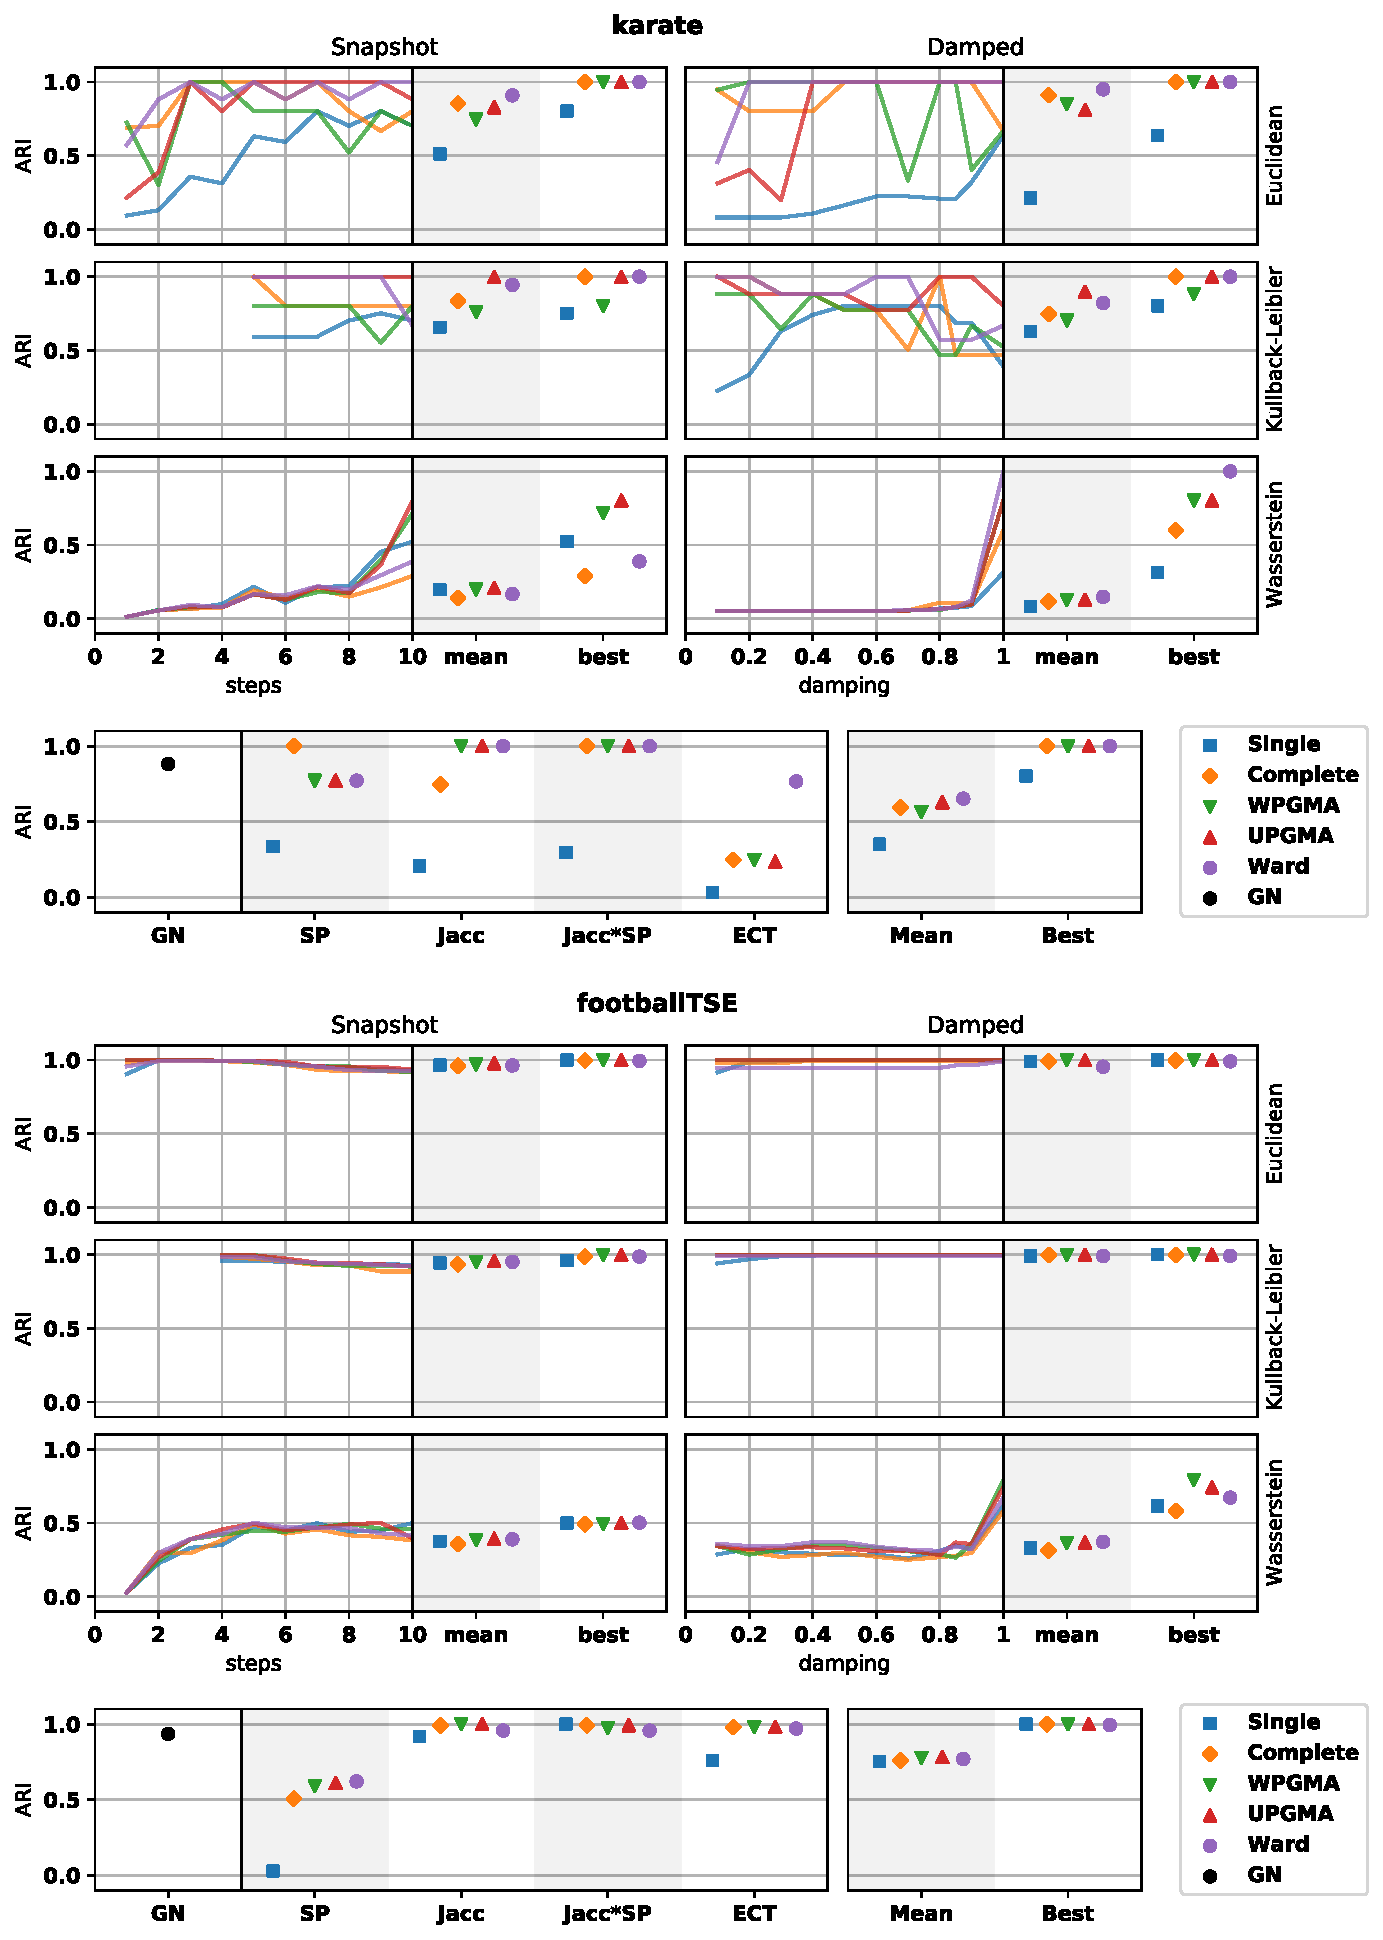
\includegraphics[height=\textheight]{power/figures/ARI1.pdf}
    \caption{Results for \texttt{karate} and \texttt{footballTSE}. Each linkage method is denoted by a different color and symbol.
    ARI is on y-axis, all clusterings on x-axis.
    Girvan-Newman is GN. Average and best ARI for all runs is in bottom right. Missing values for KL are due to probabilities of 0.}
    \label{fig:ARI1}
\end{figure}
\begin{figure}
    \centering
    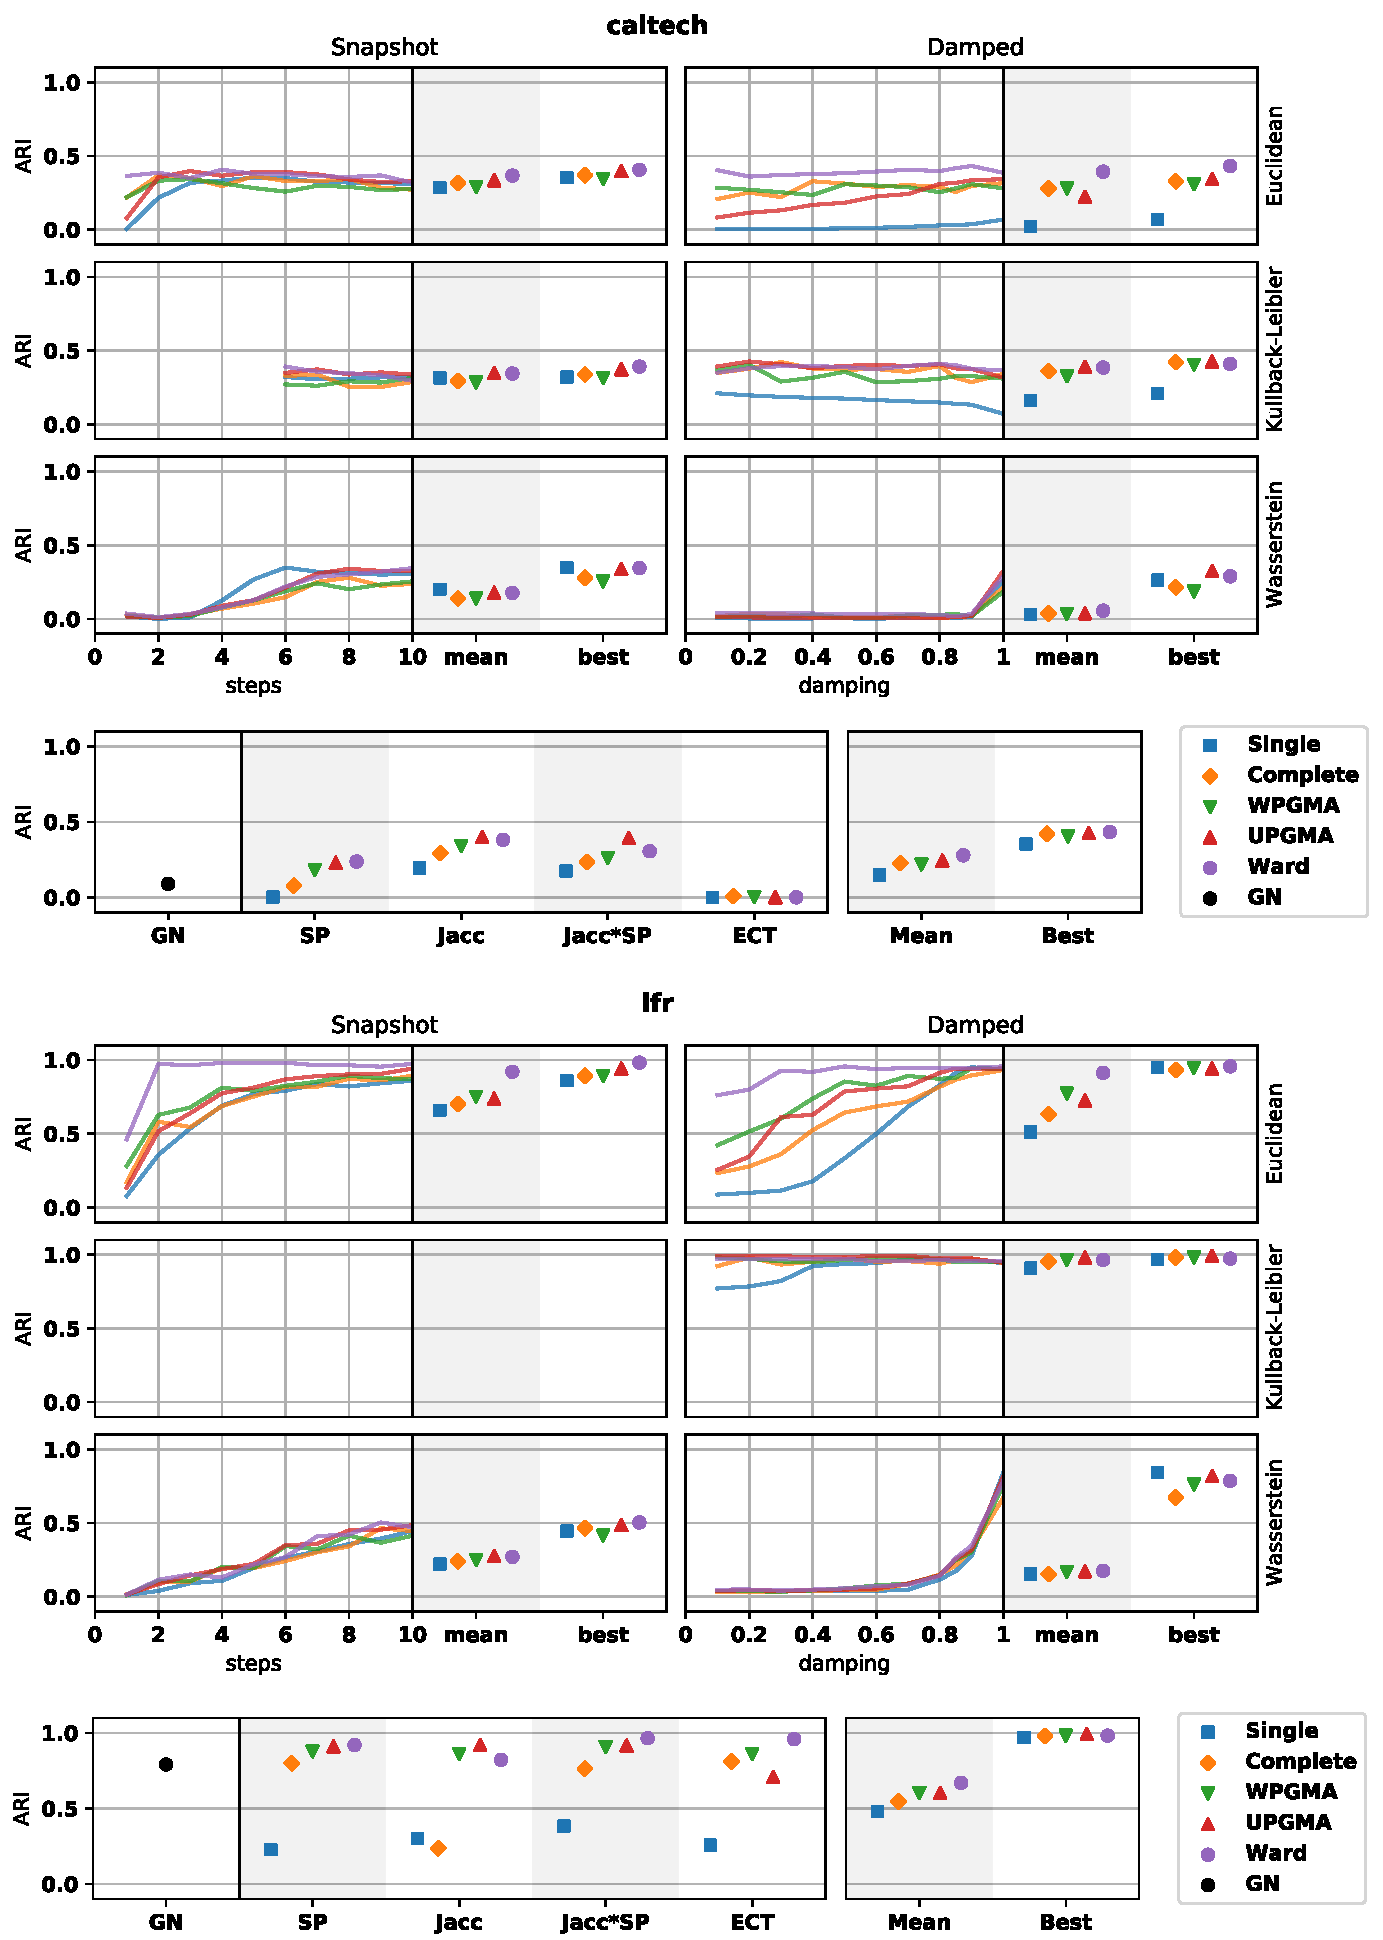
\includegraphics[height=\textheight]{power/figures/ARI2.pdf}
    \caption{Results for \texttt{caltech} and \texttt{lfr}.}
    \label{fig:ARI2}
\end{figure}

\subsubsection{Results}
The aim of this study is to answer two questions: which dissimilarity measure is best, and which linkage method is best for clustering this dissimilarity?
Unfortunately there is no clear-cut answer to either question, but the results can be interpreted to give some recommendations. Looking at the bottom right panels for each graph, it is immediately clear that single linkage is the least effective and should be avoided. The best scores for the remaining linkage methods generally hover around the same value, and so it is clear that the remaining four linkage methods all \emph{can} result in high quality results. Looking at the mean ARI scores, however, it becomes apparent that Ward's method produces the best results on average. 

% A more qualitative observation is that Ward also tends to give the best hierarchical structure in terms of neat trees without branches that, which is difficult to measure but results in the best bundles.
The best dissimilarity for Ward over all graphs is Euclidean on snapshot embedding with $t=5$ in Equation~\eqref{eq:walktrap}, and it seems the original authors in \cite{Pons2006} agree with this choice as they performed most of their analysis using the same value.
Despite being a distance metric, the performance of Wasserstein is consistently poorer than both Euclidean and KL. It is worth noting, however, that it consistently rises as the value of $t$ rises for both snapshot and damped embeddings. Both sets of parameters converge to the same 

This is what we will use for plotting results

\subsection{Pruning}
\label{sec:pruning}
The final step to producing a hierarchical edge bundling visualisation is to 
However the problem with using a dendrogram is that, as a binary tree, it contains as many branch nodes as leaves, which means that the resulting splines have far too many control points to be meaningful. An example of this can be seen in Figure~\ref{fig:lesmis}.
Jia et al.\ \cite{Jia2011} attempt to alleviate this by introducing 
but GN complexity is also ridiculous

mention the optimal ordering from Scipy, Bar-Joseph et al.\ \cite{Bar-Joseph2001}, around a circle. This could be used to, for example, optimise an edge bundling specific objective function.

merge branches in tree to make pretty (following \cite{Pons2006}), but this is not always high quality, as it can potentially merge every single 
ideally cuts can be human driven \cite{Vogogias2016}
trees can be interactively explored using \cite{Archambault2008}

optimal leaf ordering also pretty
Garland paper does pruning of top down
mention that pruning is not the only way to do things e.g. skipping more control points. YMMV


\begin{figure}
    \centering
    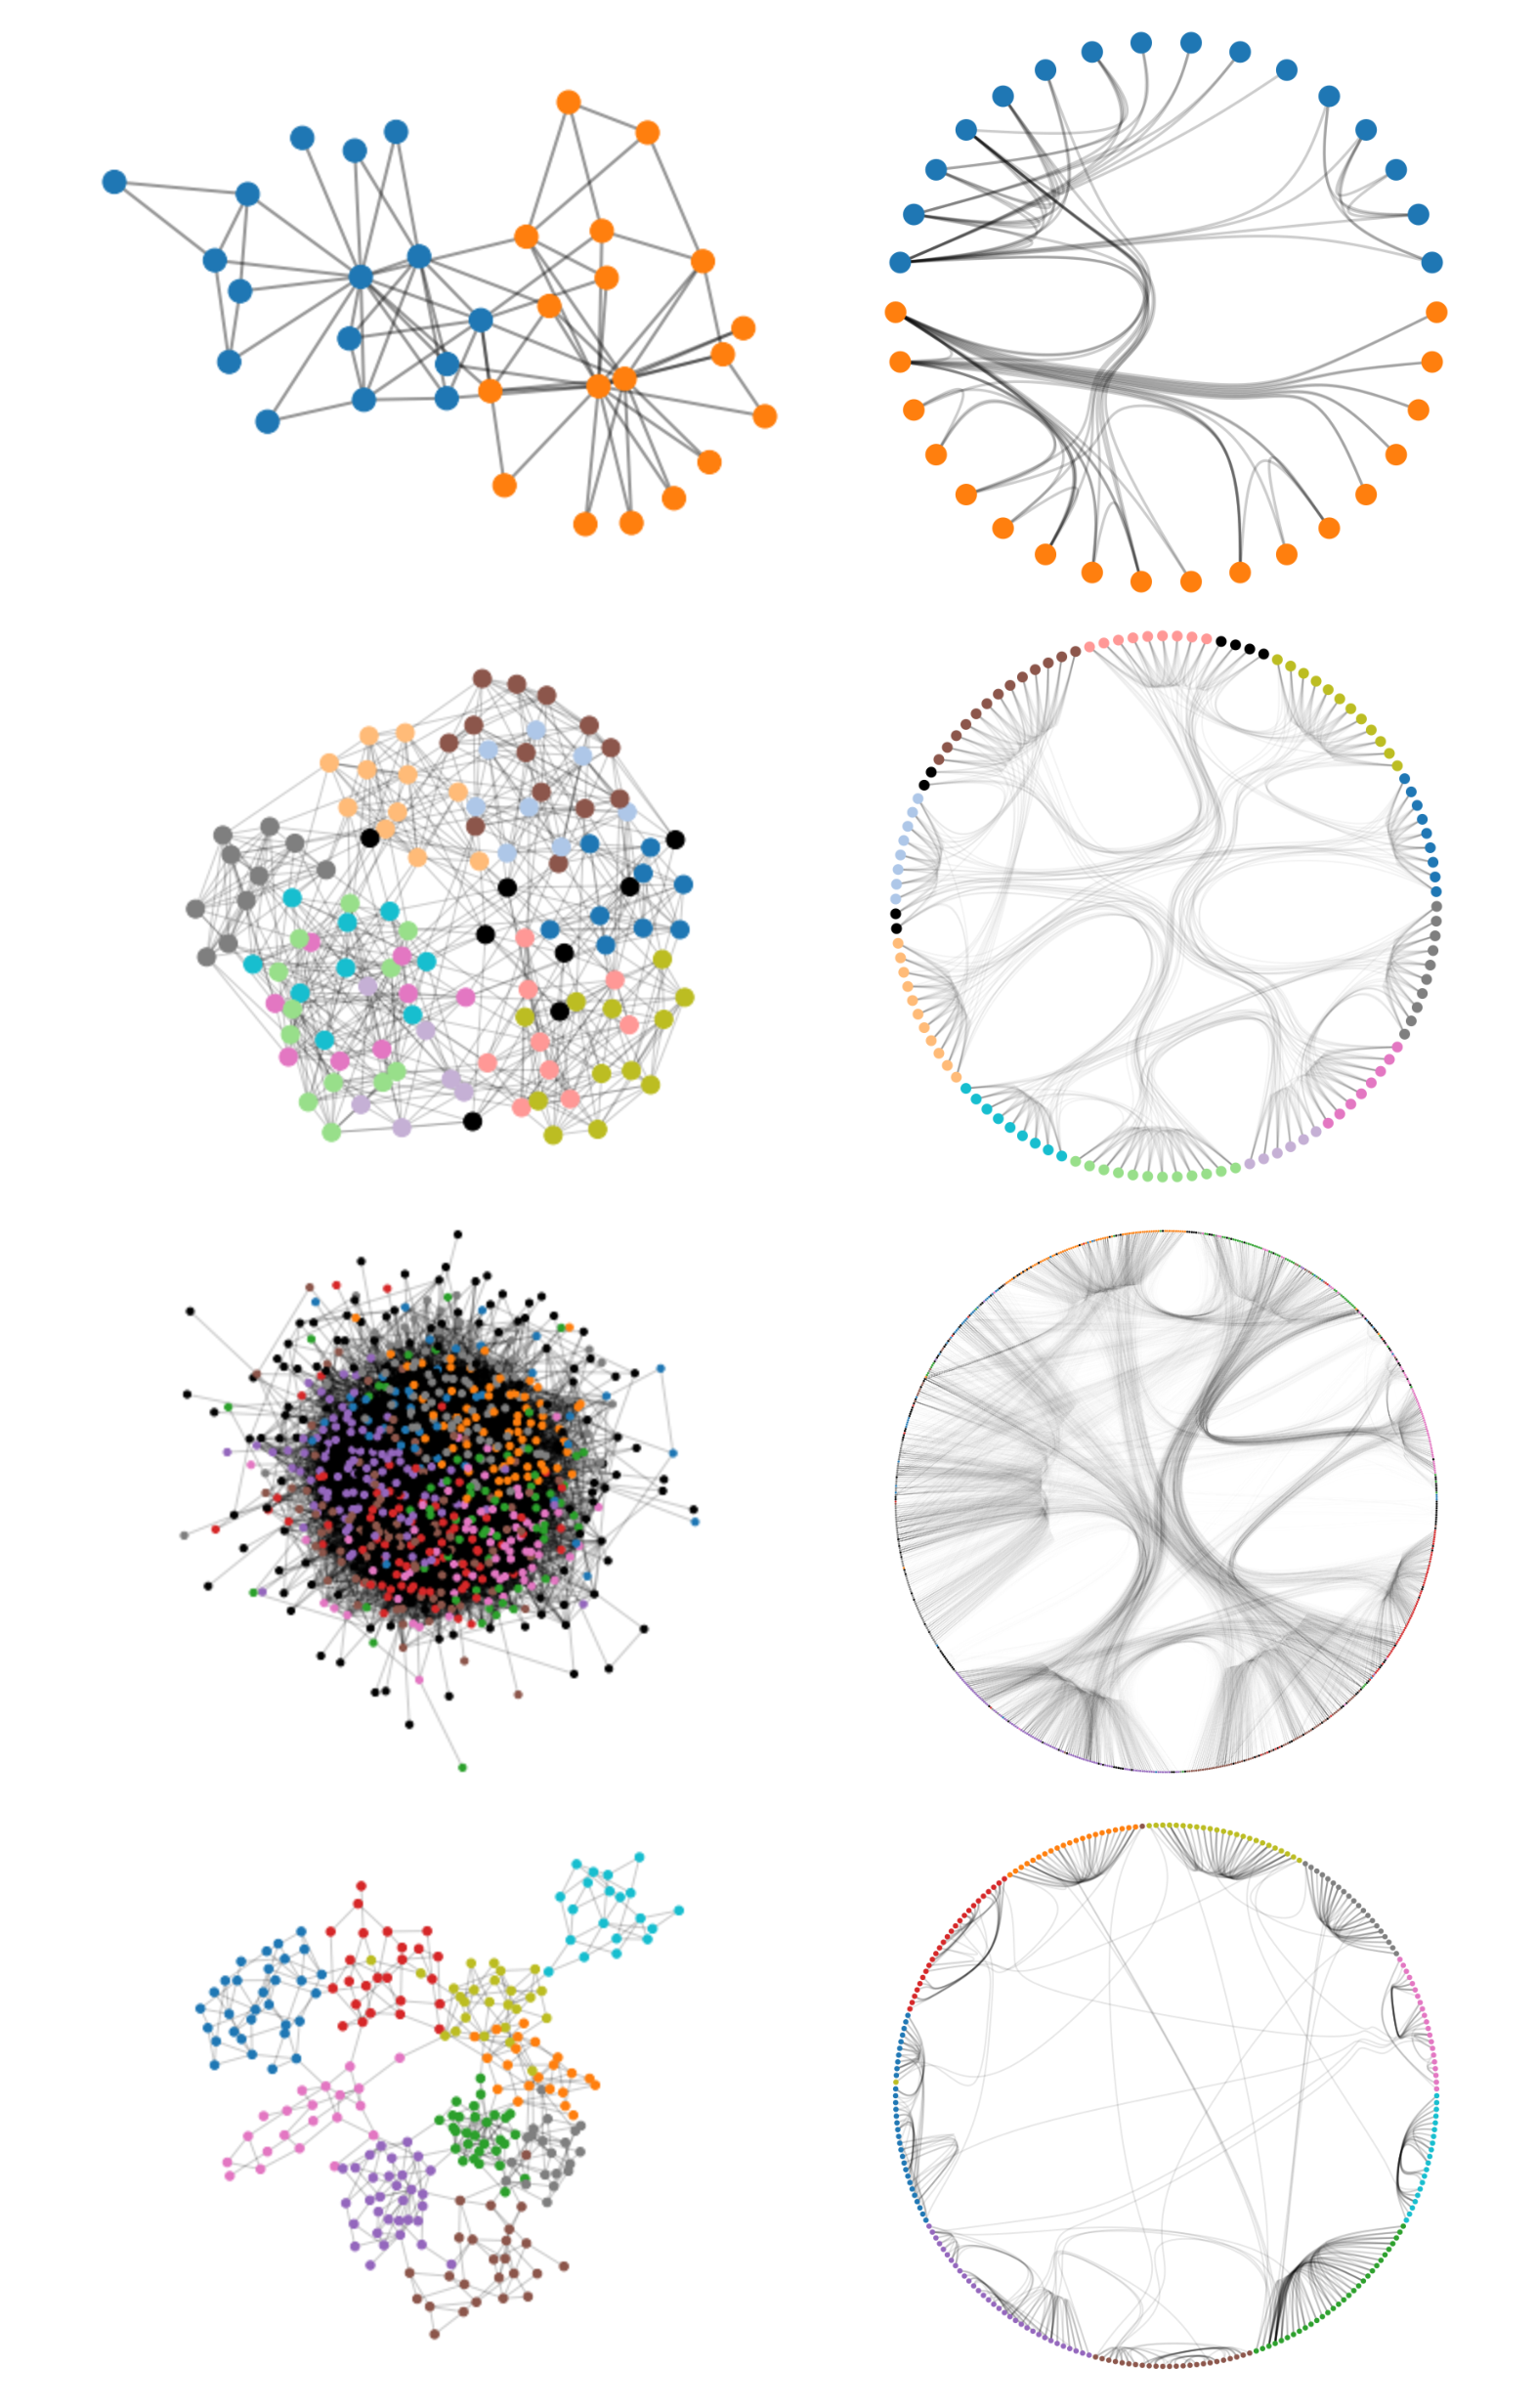
\includegraphics[height=.9\textheight]{power/figures/bundled.pdf}
    \caption{Drawings of the graphs in Table~\ref{tab:bundle_graphs} using both a stress layout (left) and with hierarchical edge bundling (right). Colours of nodes correspond to the ground truth clusters included in the data.
    For football, 8 of its teams are singleton clusters in independent divisions, and for caltech ??? are unassigned to dorms}
    \label{fig:untangled_hairballs}
\end{figure}

END THIS CHAPTER WITH PSEUDOCODE

\begin{figure}
    % \centering
    % \includegraphics{}
     \caption{TODO: show pruning example}
     \label{fig:pruning}   
\end{figure}

\begin{figure}
    \removeAlgorithmFigureError
    \DontPrintSemicolon
    \begin{algorithm}[H]
    \SetKwInOut{Input}{inputs}
    \SetKwInOut{Output}{output}
    \SetKwFor{ForEach}{foreach}{}{}
    \SetKwRepeat{Do}{do}{while}
    \SetKwIF{If}{ElseIf}{Else}{if}{}{else if}{else}{}
    \Input{graph $G=(V,E)$}
    \Output{drawing $A$}
    
    $M \leftarrow \{(\emptyset,\,N(v))\ |\ v\in V\}$
    
    \Do{$\kappa_\text{best}>0$}{
        $\kappa_\text{best}\leftarrow0$
        
        \ForEach{\emph{pair of modules} $\{m,n\}\in M_\text{top}\times M_\text{top}$}{
        \label{pseudo:top}
            $\kappa_\text{best} \leftarrow \max(\kappa(m,n),\,\kappa_\text{best})$
            \label{pseudo:kappa}
        }
        $\textsc{merge}(\{m,n\}_\text{best})$
        \label{pseudo:merge}
    }
    
    \caption{\textsc{Hierarchical Edge Bundling}}
    \label{algo:heb}
    \end{algorithm}
    \caption{hi}
    \label{pgd_pseudo}
\end{figure} 

\subsection{Discussion}
Girvan-Newman has a higher runtime complexity. Calculating betweenness-centrality is $\mathcal{O}(|V||E|)$ \cite{Brandes2001a}. Since this must be done within 
but this is all kind of besides the point for HEB because the kind of structure we want to reveal is not clique structure, but biclique structure.
% it is very important to realise that there are two types of clusters, which will be henceforth referred to as 'community' and 'betweenness' structure. This can also be referred to as 'assortative' and 'disassortative'.
% some networks have both at the same time, and it is therefore difficult
In any case, this is a small test set and the correct 
Applying hierarchical edge bundles to the test set leads to smaller edges being within clusters and larger ones being across the 

% Another benefit to agglomerative methods is that it is easy to interpret and understand what the algorithm is doing, even if the answer is suboptimal. I would always pick an algorithm that I fully understand for a visualisation over a black-box algorithm that produces slightly better results. But this is just opinion.

interaction is MEGA IMPORTANT. Being able to switch between different bundles and see where each node goes interactively is the only way these. A possible study to test the actual effectiveness of bundles could be to ask participants to try and identify ground truth cliques and/or bicliques from different bundling configurations.
For a practitioner, this kind of technique depends greatly on the data input.

\section{Power-confluent Drawings}
\begin{figure}
    \caption{TODO: teaser image in pconfluent paper}
    \label{fig:power_teaser}
\end{figure}
in confluent drawings the aforementioned trade-off is actually attempted to be avoided
it is likened to lossless compression.

2 parts: finding the power groups, then converting to a confluent drawing. The results here improve the speed and quality of the first part, and fix theoretical issues with the second.
The nested structure of power-groups is hierarchical, and so an agglomerative method is used.
\subsection{Splines}
b-spline algorithms and things
holten qualitatively said some desirable properties of b-splines, but the real benefit of them is the convex hull property, which helps to prevent crossings (explain why... because)
The importance of this has been crucially missing in the literature
examples of splines that are not convex hull is like the garland paper.
